\PassOptionsToPackage{unicode=true}{hyperref} % options for packages loaded elsewhere
\PassOptionsToPackage{hyphens}{url}
%
\documentclass[]{book}
\usepackage{lmodern}
\usepackage{amssymb,amsmath}
\usepackage{ifxetex,ifluatex}
\usepackage{fixltx2e} % provides \textsubscript
\ifnum 0\ifxetex 1\fi\ifluatex 1\fi=0 % if pdftex
  \usepackage[T1]{fontenc}
  \usepackage[utf8]{inputenc}
  \usepackage{textcomp} % provides euro and other symbols
\else % if luatex or xelatex
  \usepackage{unicode-math}
  \defaultfontfeatures{Ligatures=TeX,Scale=MatchLowercase}
\fi
% use upquote if available, for straight quotes in verbatim environments
\IfFileExists{upquote.sty}{\usepackage{upquote}}{}
% use microtype if available
\IfFileExists{microtype.sty}{%
\usepackage[]{microtype}
\UseMicrotypeSet[protrusion]{basicmath} % disable protrusion for tt fonts
}{}
\IfFileExists{parskip.sty}{%
\usepackage{parskip}
}{% else
\setlength{\parindent}{0pt}
\setlength{\parskip}{6pt plus 2pt minus 1pt}
}
\usepackage{hyperref}
\hypersetup{
            pdftitle={Introduction to Data Science with R},
            pdfborder={0 0 0},
            breaklinks=true}
\urlstyle{same}  % don't use monospace font for urls
\usepackage{color}
\usepackage{fancyvrb}
\newcommand{\VerbBar}{|}
\newcommand{\VERB}{\Verb[commandchars=\\\{\}]}
\DefineVerbatimEnvironment{Highlighting}{Verbatim}{commandchars=\\\{\}}
% Add ',fontsize=\small' for more characters per line
\usepackage{framed}
\definecolor{shadecolor}{RGB}{248,248,248}
\newenvironment{Shaded}{\begin{snugshade}}{\end{snugshade}}
\newcommand{\AlertTok}[1]{\textcolor[rgb]{0.94,0.16,0.16}{#1}}
\newcommand{\AnnotationTok}[1]{\textcolor[rgb]{0.56,0.35,0.01}{\textbf{\textit{#1}}}}
\newcommand{\AttributeTok}[1]{\textcolor[rgb]{0.77,0.63,0.00}{#1}}
\newcommand{\BaseNTok}[1]{\textcolor[rgb]{0.00,0.00,0.81}{#1}}
\newcommand{\BuiltInTok}[1]{#1}
\newcommand{\CharTok}[1]{\textcolor[rgb]{0.31,0.60,0.02}{#1}}
\newcommand{\CommentTok}[1]{\textcolor[rgb]{0.56,0.35,0.01}{\textit{#1}}}
\newcommand{\CommentVarTok}[1]{\textcolor[rgb]{0.56,0.35,0.01}{\textbf{\textit{#1}}}}
\newcommand{\ConstantTok}[1]{\textcolor[rgb]{0.00,0.00,0.00}{#1}}
\newcommand{\ControlFlowTok}[1]{\textcolor[rgb]{0.13,0.29,0.53}{\textbf{#1}}}
\newcommand{\DataTypeTok}[1]{\textcolor[rgb]{0.13,0.29,0.53}{#1}}
\newcommand{\DecValTok}[1]{\textcolor[rgb]{0.00,0.00,0.81}{#1}}
\newcommand{\DocumentationTok}[1]{\textcolor[rgb]{0.56,0.35,0.01}{\textbf{\textit{#1}}}}
\newcommand{\ErrorTok}[1]{\textcolor[rgb]{0.64,0.00,0.00}{\textbf{#1}}}
\newcommand{\ExtensionTok}[1]{#1}
\newcommand{\FloatTok}[1]{\textcolor[rgb]{0.00,0.00,0.81}{#1}}
\newcommand{\FunctionTok}[1]{\textcolor[rgb]{0.00,0.00,0.00}{#1}}
\newcommand{\ImportTok}[1]{#1}
\newcommand{\InformationTok}[1]{\textcolor[rgb]{0.56,0.35,0.01}{\textbf{\textit{#1}}}}
\newcommand{\KeywordTok}[1]{\textcolor[rgb]{0.13,0.29,0.53}{\textbf{#1}}}
\newcommand{\NormalTok}[1]{#1}
\newcommand{\OperatorTok}[1]{\textcolor[rgb]{0.81,0.36,0.00}{\textbf{#1}}}
\newcommand{\OtherTok}[1]{\textcolor[rgb]{0.56,0.35,0.01}{#1}}
\newcommand{\PreprocessorTok}[1]{\textcolor[rgb]{0.56,0.35,0.01}{\textit{#1}}}
\newcommand{\RegionMarkerTok}[1]{#1}
\newcommand{\SpecialCharTok}[1]{\textcolor[rgb]{0.00,0.00,0.00}{#1}}
\newcommand{\SpecialStringTok}[1]{\textcolor[rgb]{0.31,0.60,0.02}{#1}}
\newcommand{\StringTok}[1]{\textcolor[rgb]{0.31,0.60,0.02}{#1}}
\newcommand{\VariableTok}[1]{\textcolor[rgb]{0.00,0.00,0.00}{#1}}
\newcommand{\VerbatimStringTok}[1]{\textcolor[rgb]{0.31,0.60,0.02}{#1}}
\newcommand{\WarningTok}[1]{\textcolor[rgb]{0.56,0.35,0.01}{\textbf{\textit{#1}}}}
\usepackage{longtable,booktabs}
% Fix footnotes in tables (requires footnote package)
\IfFileExists{footnote.sty}{\usepackage{footnote}\makesavenoteenv{longtable}}{}
\usepackage{graphicx,grffile}
\makeatletter
\def\maxwidth{\ifdim\Gin@nat@width>\linewidth\linewidth\else\Gin@nat@width\fi}
\def\maxheight{\ifdim\Gin@nat@height>\textheight\textheight\else\Gin@nat@height\fi}
\makeatother
% Scale images if necessary, so that they will not overflow the page
% margins by default, and it is still possible to overwrite the defaults
% using explicit options in \includegraphics[width, height, ...]{}
\setkeys{Gin}{width=\maxwidth,height=\maxheight,keepaspectratio}
\setlength{\emergencystretch}{3em}  % prevent overfull lines
\providecommand{\tightlist}{%
  \setlength{\itemsep}{0pt}\setlength{\parskip}{0pt}}
\setcounter{secnumdepth}{5}
% Redefines (sub)paragraphs to behave more like sections
\ifx\paragraph\undefined\else
\let\oldparagraph\paragraph
\renewcommand{\paragraph}[1]{\oldparagraph{#1}\mbox{}}
\fi
\ifx\subparagraph\undefined\else
\let\oldsubparagraph\subparagraph
\renewcommand{\subparagraph}[1]{\oldsubparagraph{#1}\mbox{}}
\fi

% set default figure placement to htbp
\makeatletter
\def\fps@figure{htbp}
\makeatother

\usepackage{etoolbox}
\makeatletter
\providecommand{\subtitle}[1]{% add subtitle to \maketitle
  \apptocmd{\@title}{\par {\large #1 \par}}{}{}
}
\makeatother
\usepackage{booktabs}
% https://github.com/rstudio/rmarkdown/issues/337
\let\rmarkdownfootnote\footnote%
\def\footnote{\protect\rmarkdownfootnote}

% https://github.com/rstudio/rmarkdown/pull/252
\usepackage{titling}
\setlength{\droptitle}{-2em}

\pretitle{\vspace{\droptitle}\centering\huge}
\posttitle{\par}

\preauthor{\centering\large\emph}
\postauthor{\par}

\predate{\centering\large\emph}
\postdate{\par}
\usepackage[]{natbib}
\bibliographystyle{apalike}

\title{Introduction to Data Science with R}
\author{true \and true \and true}
\date{2019-11-27}

\begin{document}
\maketitle

{
\setcounter{tocdepth}{1}
\tableofcontents
}
\hypertarget{knowledge-is-sharing.}{%
\chapter{Knowledge is sharing.}\label{knowledge-is-sharing.}}

This is a \emph{sample} book written in \textbf{Markdown}. You can use anything that Pandoc's Markdown supports, e.g., a math equation \(a^2 + b^2 = c^2\).

The \textbf{bookdown} package can be installed from CRAN or Github:

\begin{Shaded}
\begin{Highlighting}[]
\KeywordTok{install.packages}\NormalTok{(}\StringTok{"bookdown"}\NormalTok{)}
\CommentTok{# or the development version}
\CommentTok{# devtools::install_github("rstudio/bookdown")}
\end{Highlighting}
\end{Shaded}

Remember each Rmd file contains one and only one chapter, and a chapter is defined by the first-level heading \texttt{\#}.

To compile this example to PDF, you need XeLaTeX. You are recommended to install TinyTeX (which includes XeLaTeX): \url{https://yihui.org/tinytex/}.

\hypertarget{think-about-your-end-before-your-start}{%
\chapter{Think about your end before your start}\label{think-about-your-end-before-your-start}}

You can label chapter and section titles using \texttt{\{\#label\}} after them, e.g., we can reference Chapter \ref{intro}. If you do not manually label them, there will be automatic labels anyway, e.g., Chapter \ref{methods}.

Figures and tables with captions will be placed in \texttt{figure} and \texttt{table} environments, respectively.

\begin{Shaded}
\begin{Highlighting}[]
\KeywordTok{par}\NormalTok{(}\DataTypeTok{mar =} \KeywordTok{c}\NormalTok{(}\DecValTok{4}\NormalTok{, }\DecValTok{4}\NormalTok{, }\FloatTok{.1}\NormalTok{, }\FloatTok{.1}\NormalTok{))}
\KeywordTok{plot}\NormalTok{(pressure, }\DataTypeTok{type =} \StringTok{'b'}\NormalTok{, }\DataTypeTok{pch =} \DecValTok{19}\NormalTok{)}
\end{Highlighting}
\end{Shaded}

\begin{figure}

{\centering 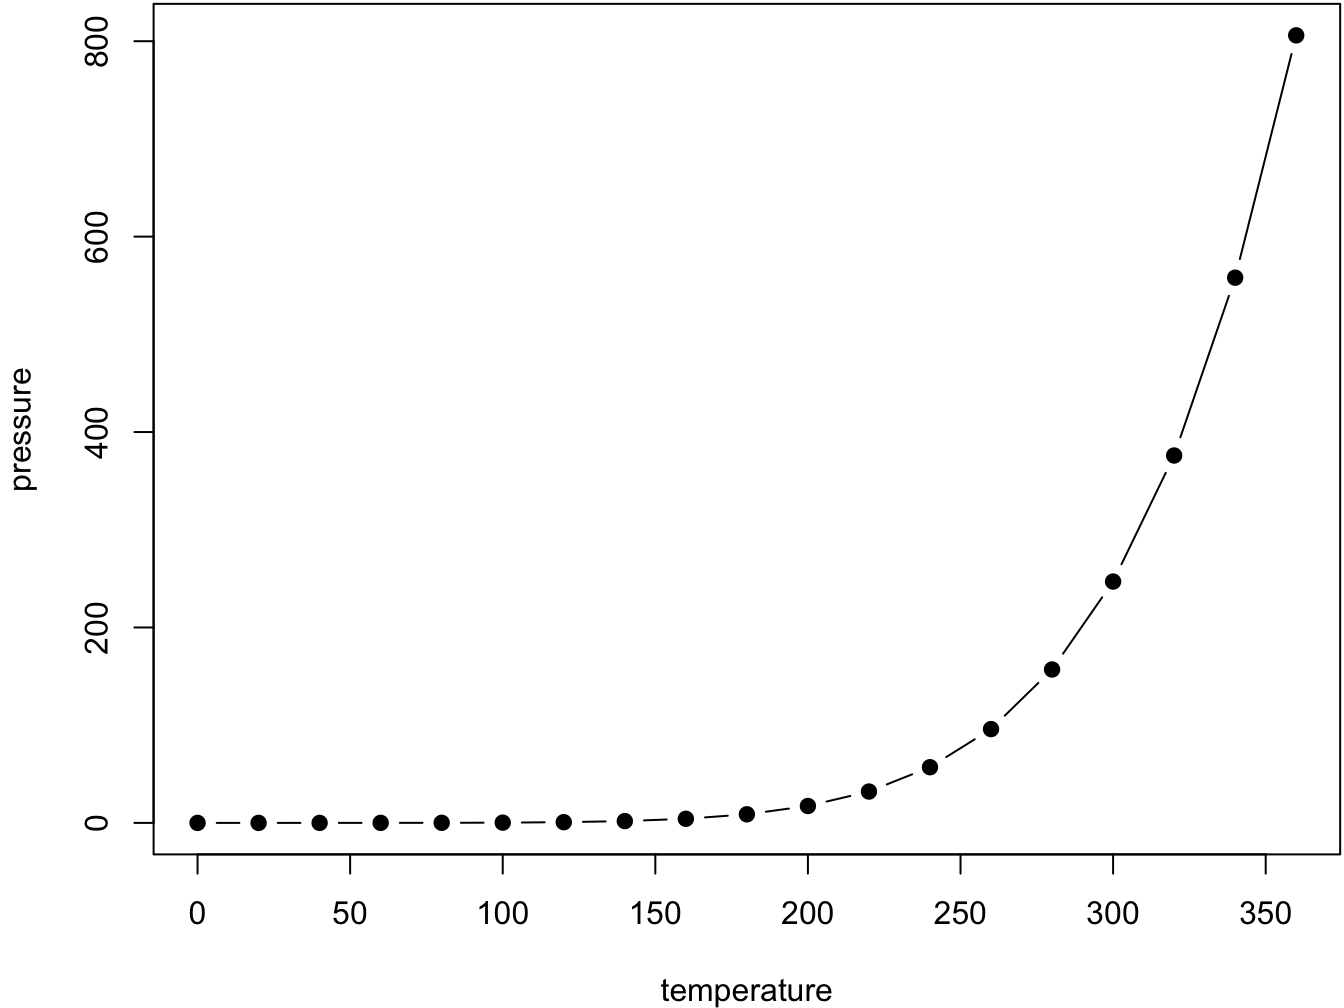
\includegraphics[width=0.8\linewidth]{R_DE_files/figure-latex/nice-fig-1} 

}

\caption{Here is a nice figure!}\label{fig:nice-fig}
\end{figure}

Reference a figure by its code chunk label with the \texttt{fig:} prefix, e.g., see Figure \ref{fig:nice-fig}. Similarly, you can reference tables generated from \texttt{knitr::kable()}, e.g., see Table \ref{tab:nice-tab}.

\begin{Shaded}
\begin{Highlighting}[]
\NormalTok{knitr}\OperatorTok{::}\KeywordTok{kable}\NormalTok{(}
  \KeywordTok{head}\NormalTok{(iris, }\DecValTok{20}\NormalTok{), }\DataTypeTok{caption =} \StringTok{'Here is a nice table!'}\NormalTok{,}
  \DataTypeTok{booktabs =} \OtherTok{TRUE}
\NormalTok{)}
\end{Highlighting}
\end{Shaded}

\begin{table}

\caption{\label{tab:nice-tab}Here is a nice table!}
\centering
\begin{tabular}[t]{rrrrl}
\toprule
Sepal.Length & Sepal.Width & Petal.Length & Petal.Width & Species\\
\midrule
5.1 & 3.5 & 1.4 & 0.2 & setosa\\
4.9 & 3.0 & 1.4 & 0.2 & setosa\\
4.7 & 3.2 & 1.3 & 0.2 & setosa\\
4.6 & 3.1 & 1.5 & 0.2 & setosa\\
5.0 & 3.6 & 1.4 & 0.2 & setosa\\
\addlinespace
5.4 & 3.9 & 1.7 & 0.4 & setosa\\
4.6 & 3.4 & 1.4 & 0.3 & setosa\\
5.0 & 3.4 & 1.5 & 0.2 & setosa\\
4.4 & 2.9 & 1.4 & 0.2 & setosa\\
4.9 & 3.1 & 1.5 & 0.1 & setosa\\
\addlinespace
5.4 & 3.7 & 1.5 & 0.2 & setosa\\
4.8 & 3.4 & 1.6 & 0.2 & setosa\\
4.8 & 3.0 & 1.4 & 0.1 & setosa\\
4.3 & 3.0 & 1.1 & 0.1 & setosa\\
5.8 & 4.0 & 1.2 & 0.2 & setosa\\
\addlinespace
5.7 & 4.4 & 1.5 & 0.4 & setosa\\
5.4 & 3.9 & 1.3 & 0.4 & setosa\\
5.1 & 3.5 & 1.4 & 0.3 & setosa\\
5.7 & 3.8 & 1.7 & 0.3 & setosa\\
5.1 & 3.8 & 1.5 & 0.3 & setosa\\
\bottomrule
\end{tabular}
\end{table}

You can write citations, too. For example, we are using the \textbf{bookdown} package \citep{R-bookdown} in this sample book, which was built on top of R Markdown and \textbf{knitr} \citep{xie2015}.

\hypertarget{documentation---bookdown-styled}{%
\chapter{Documentation - bookdown-styled}\label{documentation---bookdown-styled}}

First, choose \emph{New Project} and \emph{New Directiory}.

Second, choose \emph{Book Project using bookdown} and pick a name as well as your preferred directory. RStudio will automatically set up the Rproj as well as the folder skeleton.

Third, tie the existing project with Git through the \texttt{usethis} package. It will re-organise the existing project folder and prepare the Git integration.

\begin{Shaded}
\begin{Highlighting}[]
\OperatorTok{>}\StringTok{ }\NormalTok{usethis}\OperatorTok{::}\KeywordTok{use_git}\NormalTok{()}

\NormalTok{✔ Setting active project to }\StringTok{'/Users/sushicat/Dropbox/R_Me/R_DE'}
\NormalTok{✔ Initialising Git repo}
\NormalTok{✔ Adding }\StringTok{'.Rhistory'}\NormalTok{, }\StringTok{'.RData'}\NormalTok{, }\StringTok{'.Rproj.user'}\NormalTok{ to }\StringTok{'.gitignore'}
\NormalTok{There are }\DecValTok{15}\NormalTok{ uncommitted files}\OperatorTok{:}
\ErrorTok{*}\StringTok{ '_bookdown.yml'}
\OperatorTok{*}\StringTok{ '_output.yml'}
\OperatorTok{*}\StringTok{ '.gitignore'}
\OperatorTok{*}\StringTok{ '01-intro.Rmd'}
\OperatorTok{*}\StringTok{ '02-literature.Rmd'}
\OperatorTok{*}\StringTok{ '03-method.Rmd'}
\OperatorTok{*}\StringTok{ '04-application.Rmd'}
\OperatorTok{*}\StringTok{ '05-summary.Rmd'}
\OperatorTok{*}\StringTok{ '06-references.Rmd'}
\OperatorTok{*}\StringTok{ 'book.bib'}
\OperatorTok{*}\StringTok{ 'index.Rmd'}
\OperatorTok{*}\StringTok{ 'preamble.tex'}
\OperatorTok{*}\StringTok{ 'R_DE.Rproj'}
\OperatorTok{*}\StringTok{ 'README.md'}
\OperatorTok{*}\StringTok{ 'style.css'}
\NormalTok{Is it ok to commit them?}

\DecValTok{1}\OperatorTok{:}\StringTok{ }\NormalTok{Not now}
\DecValTok{2}\OperatorTok{:}\StringTok{ }\NormalTok{For sure}
\DecValTok{3}\OperatorTok{:}\StringTok{ }\NormalTok{No way}

\NormalTok{Selection}\OperatorTok{:}\StringTok{ }\DecValTok{2}
\NormalTok{✔ Adding files}
\NormalTok{✔ Commit with message }\StringTok{'Initial commit'}
\NormalTok{● A restart of RStudio is required to activate the Git pane}
\NormalTok{Restart now?}

\DecValTok{1}\OperatorTok{:}\StringTok{ }\NormalTok{Not now}
\DecValTok{2}\OperatorTok{:}\StringTok{ }\NormalTok{Yup}
\DecValTok{3}\OperatorTok{:}\StringTok{ }\NormalTok{Absolutely not}

\NormalTok{Selection}\OperatorTok{:}\StringTok{ }\DecValTok{2}
\end{Highlighting}
\end{Shaded}

Fourth, create a GitHub repo through the \texttt{usethis} package and if the project name is available on the owner's repos. When facing git protocol, choose \texttt{https}.

\begin{Shaded}
\begin{Highlighting}[]
\OperatorTok{>}\StringTok{ }\NormalTok{usethis}\OperatorTok{::}\KeywordTok{use_github}\NormalTok{()}

\NormalTok{✔ Setting active project to }\StringTok{'/Users/sushicat/Dropbox/R_Me/R_DE'}
\NormalTok{✔ Checking that current branch is }\StringTok{'master'}
\NormalTok{Which git protocol to use? (enter }\DecValTok{0}\NormalTok{ to exit) }

\DecValTok{1}\OperatorTok{:}\StringTok{ }\NormalTok{ssh   <-}\OperatorTok{-}\StringTok{ }\NormalTok{presumes that you have set up ssh keys}
\DecValTok{2}\OperatorTok{:}\StringTok{ }\NormalTok{https <-}\OperatorTok{-}\StringTok{ }\NormalTok{choose this }\ControlFlowTok{if}\NormalTok{ you don}\StringTok{'t have ssh keys (or don'}\NormalTok{t know }\ControlFlowTok{if}\NormalTok{ you do}\ErrorTok{)}

\NormalTok{Selection}\OperatorTok{:}\StringTok{ }\DecValTok{2}
\NormalTok{● Tip}\OperatorTok{:}\StringTok{ }\NormalTok{To suppress this menu }\ControlFlowTok{in}\NormalTok{ future, put}
  \StringTok{`}\DataTypeTok{options(usethis.protocol = "https")}\StringTok{`}
  \ControlFlowTok{in}\NormalTok{ your script or }\ControlFlowTok{in}\NormalTok{ a user}\OperatorTok{-}\StringTok{ }\NormalTok{or project}\OperatorTok{-}\NormalTok{level startup file, }\StringTok{'.Rprofile'}\NormalTok{.}
\NormalTok{  Call }\StringTok{`}\DataTypeTok{usethis::edit_r_profile()}\StringTok{`}\NormalTok{ to open it }\ControlFlowTok{for}\NormalTok{ editing.}
\NormalTok{● Check title and description}
\NormalTok{  Name}\OperatorTok{:}\StringTok{        }\NormalTok{Bradford}
\NormalTok{  Description}\OperatorTok{:}\StringTok{ }
\NormalTok{Are title and description ok?}

\DecValTok{1}\OperatorTok{:}\StringTok{ }\NormalTok{Yeah}
\DecValTok{2}\OperatorTok{:}\StringTok{ }\NormalTok{Not now}
\DecValTok{3}\OperatorTok{:}\StringTok{ }\NormalTok{Absolutely not}

\NormalTok{Selection}\OperatorTok{:}\StringTok{ }\DecValTok{1}
\NormalTok{✔ Creating GitHub repository}
\NormalTok{✔ Setting remote }\StringTok{'origin'}\NormalTok{ to }\StringTok{'https://github.com/dataning/R_DE.git'}
\NormalTok{✔ Pushing }\StringTok{'master'}\NormalTok{ branch to GitHub and setting remote tracking branch}
\NormalTok{✔ Opening URL }\StringTok{'https://github.com/dataning/R_DE'}
\end{Highlighting}
\end{Shaded}

Fifth, create and save a random R.script in the current project. The commit and push the change of the project to your GitHub repo. You can go to your GitHub repo and check if the R script has been added. This should tell you whether your Rproj and GitHub Repo are fully synced/integrated.

Sixth, go to Netlify and deploy your GitHub repo on Netlify. This will give you the ability to perform continuous deployment as well as deployment to custom domain.

Type in your Rpoj's GitHub repo name.

You need to put down \texttt{\_book} in \emph{Publish directory}.

\hypertarget{elastigirl-is-here}{%
\chapter{Elastigirl is Here}\label{elastigirl-is-here}}

\begin{quote}
When designing the Incredible family, Brad Bird wanted each of their superpowers to be related to their personality. He felt that as a mother, Helen was required by society to be pulled in many different directions, which led to her being given an elastic ability.
\end{quote}

The same we can say to all sort of data science projects. We are always required by different stakeholders to be pull in many different directions. For us, we have to nail down where we are and how to initiate a new project first.

First of all, we find where we stand.

\begin{Shaded}
\begin{Highlighting}[]
\OperatorTok{>}\StringTok{ }\NormalTok{here}\OperatorTok{::}\KeywordTok{here}\NormalTok{()}

\NormalTok{[}\DecValTok{1}\NormalTok{] }\StringTok{"/Users/sushicat/Dropbox/R_Me/Hero_book"}
\end{Highlighting}
\end{Shaded}

Second, we find out what we are being surrounded.

\begin{Shaded}
\begin{Highlighting}[]
\OperatorTok{>}\StringTok{ }\NormalTok{fs}\OperatorTok{::}\KeywordTok{dir_ls}\NormalTok{()}

\DecValTok{01}\OperatorTok{-}\NormalTok{think.Rmd           }\DecValTok{02}\OperatorTok{-}\NormalTok{pm.Rmd              }\DecValTok{03}\OperatorTok{-}\NormalTok{load}\OperatorTok{-}\NormalTok{data.Rmd       }\DecValTok{04}\OperatorTok{-}\NormalTok{tidy}\OperatorTok{-}\NormalTok{data.Rmd       }
\DecValTok{05}\OperatorTok{-}\NormalTok{bayesian.Rmd        }\DecValTok{06}\OperatorTok{-}\NormalTok{Elastigirl_}\FloatTok{1.}\NormalTok{Rmd }\DecValTok{06}\NormalTok{_Elastigirl_}\FloatTok{1.}\NormalTok{R   }\DecValTok{20}\OperatorTok{-}\NormalTok{references.Rmd      }
\NormalTok{CreditCard             Creditcard_hack.R      Data                   Hero_book.Rproj        }
\NormalTok{Hero_book.log          README.md              _book                  _bookdown.yml          }
\NormalTok{_bookdown_files        _output.yml            book.bib               index.Rmd              }
\NormalTok{packages.bib           preamble.tex           style.css }
\end{Highlighting}
\end{Shaded}

Third, we pick somewhere (in this case - the data folder) to explore further.

\begin{Shaded}
\begin{Highlighting}[]
\OperatorTok{>}\StringTok{ }\NormalTok{fs}\OperatorTok{::}\KeywordTok{dir_ls}\NormalTok{(}\StringTok{"Data"}\NormalTok{)}
\OperatorTok{>}\StringTok{ }\NormalTok{fs}\OperatorTok{::}\KeywordTok{dir_ls}\NormalTok{(}\StringTok{"Data/Subway_delays"}\NormalTok{)}

\NormalTok{Data}\OperatorTok{/}\NormalTok{Subway_delays}\OperatorTok{/}\NormalTok{Subway}\OperatorTok{&}\NormalTok{SRT_Logs_April_}\FloatTok{2018.}\NormalTok{xlsx}
\NormalTok{Data}\OperatorTok{/}\NormalTok{Subway_delays}\OperatorTok{/}\NormalTok{Subway}\OperatorTok{&}\NormalTok{SRT_Logs_February_}\FloatTok{2018.}\NormalTok{xlsx}
\NormalTok{Data}\OperatorTok{/}\NormalTok{Subway_delays}\OperatorTok{/}\NormalTok{Subway}\OperatorTok{&}\NormalTok{SRT_Logs_March_}\FloatTok{2018.}\NormalTok{xlsx}
\NormalTok{Data}\OperatorTok{/}\NormalTok{Subway_delays}\OperatorTok{/}\NormalTok{Subway}\OperatorTok{&}\NormalTok{SRT_Logs_May_}\FloatTok{2018.}\NormalTok{xlsx}
\NormalTok{Data}\OperatorTok{/}\NormalTok{Subway_delays}\OperatorTok{/}\NormalTok{Subway_}\OperatorTok{&}\KeywordTok{_SRT_Logs_}\NormalTok{(August_}\DecValTok{2018}\NormalTok{).xlsx}
\NormalTok{Data}\OperatorTok{/}\NormalTok{Subway_delays}\OperatorTok{/}\NormalTok{Subway_}\OperatorTok{&}\KeywordTok{_SRT_Logs_}\NormalTok{(September_}\DecValTok{2018}\NormalTok{).xlsx}
\NormalTok{Data}\OperatorTok{/}\NormalTok{Subway_delays}\OperatorTok{/}\NormalTok{Subway_}\OperatorTok{&}\NormalTok{_SRT_Logs_December_}\FloatTok{2018.}\NormalTok{xlsx}
\NormalTok{Data}\OperatorTok{/}\NormalTok{Subway_delays}\OperatorTok{/}\NormalTok{Subway_}\OperatorTok{&}\NormalTok{_SRT_Logs_November_}\FloatTok{2018.}\NormalTok{xlsx}
\NormalTok{Data}\OperatorTok{/}\NormalTok{Subway_delays}\OperatorTok{/}\KeywordTok{Subway_SRT_Logs}\NormalTok{(January }\DecValTok{2018}\NormalTok{).xlsx}
\NormalTok{Data}\OperatorTok{/}\NormalTok{Subway_delays}\OperatorTok{/}\KeywordTok{Subway_SRT_Logs}\NormalTok{(July_}\DecValTok{2018}\NormalTok{).xlsx}
\NormalTok{Data}\OperatorTok{/}\NormalTok{Subway_delays}\OperatorTok{/}\KeywordTok{Subway_SRT_Logs}\NormalTok{(June2018).xlsx}
\NormalTok{Data}\OperatorTok{/}\NormalTok{Subway_delays}\OperatorTok{/}\KeywordTok{Subway_SRT_Logs}\NormalTok{(October }\DecValTok{2018}\NormalTok{).xlsx}
\end{Highlighting}
\end{Shaded}

Alternatively, we can use the tree strcuture to show the folder.

\begin{Shaded}
\begin{Highlighting}[]
\OperatorTok{>}\StringTok{ }\NormalTok{fs}\OperatorTok{::}\KeywordTok{dir_tree}\NormalTok{(}\StringTok{"Data/Subway_delays"}\NormalTok{)}

\NormalTok{Data}\OperatorTok{/}\NormalTok{Subway_delays}
\NormalTok{├── Subway}\OperatorTok{&}\NormalTok{SRT_Logs_April_}\FloatTok{2018.}\NormalTok{xlsx}
\NormalTok{├── Subway}\OperatorTok{&}\NormalTok{SRT_Logs_February_}\FloatTok{2018.}\NormalTok{xlsx}
\NormalTok{├── Subway}\OperatorTok{&}\NormalTok{SRT_Logs_March_}\FloatTok{2018.}\NormalTok{xlsx}
\NormalTok{├── Subway}\OperatorTok{&}\NormalTok{SRT_Logs_May_}\FloatTok{2018.}\NormalTok{xlsx}
\NormalTok{├── Subway_}\OperatorTok{&}\KeywordTok{_SRT_Logs_}\NormalTok{(August_}\DecValTok{2018}\NormalTok{).xlsx}
\NormalTok{├── Subway_}\OperatorTok{&}\KeywordTok{_SRT_Logs_}\NormalTok{(September_}\DecValTok{2018}\NormalTok{).xlsx}
\NormalTok{├── Subway_}\OperatorTok{&}\NormalTok{_SRT_Logs_December_}\FloatTok{2018.}\NormalTok{xlsx}
\NormalTok{├── Subway_}\OperatorTok{&}\NormalTok{_SRT_Logs_November_}\FloatTok{2018.}\NormalTok{xlsx}
\NormalTok{├── }\KeywordTok{Subway_SRT_Logs}\NormalTok{(January }\DecValTok{2018}\NormalTok{).xlsx}
\NormalTok{├── }\KeywordTok{Subway_SRT_Logs}\NormalTok{(July_}\DecValTok{2018}\NormalTok{).xlsx}
\NormalTok{├── }\KeywordTok{Subway_SRT_Logs}\NormalTok{(June2018).xlsx}
\NormalTok{└── }\KeywordTok{Subway_SRT_Logs}\NormalTok{(October }\DecValTok{2018}\NormalTok{).xlsx}
\end{Highlighting}
\end{Shaded}

Fourth, we make a shortcut if this is where we'd like to use or come back later.

\begin{Shaded}
\begin{Highlighting}[]
\OperatorTok{>}\StringTok{ }\NormalTok{fs}\OperatorTok{::}\KeywordTok{dir_tree}\NormalTok{(here}\OperatorTok{::}\KeywordTok{here}\NormalTok{(}\StringTok{"Data"}\NormalTok{, }\StringTok{"Subway_delays"}\NormalTok{))}

\OperatorTok{/}\NormalTok{Users}\OperatorTok{/}\NormalTok{goal}\OperatorTok{/}\NormalTok{Dropbox}\OperatorTok{/}\NormalTok{R_Me}\OperatorTok{/}\NormalTok{Hero_book}\OperatorTok{/}\NormalTok{Data}\OperatorTok{/}\NormalTok{Subway_delays}
\NormalTok{├── Subway}\OperatorTok{&}\NormalTok{SRT_Logs_April_}\FloatTok{2018.}\NormalTok{xlsx}
\NormalTok{├── Subway}\OperatorTok{&}\NormalTok{SRT_Logs_February_}\FloatTok{2018.}\NormalTok{xlsx}
\NormalTok{├── Subway}\OperatorTok{&}\NormalTok{SRT_Logs_March_}\FloatTok{2018.}\NormalTok{xlsx}
\NormalTok{├── Subway}\OperatorTok{&}\NormalTok{SRT_Logs_May_}\FloatTok{2018.}\NormalTok{xlsx}
\NormalTok{├── Subway_}\OperatorTok{&}\KeywordTok{_SRT_Logs_}\NormalTok{(August_}\DecValTok{2018}\NormalTok{).xlsx}
\NormalTok{├── Subway_}\OperatorTok{&}\KeywordTok{_SRT_Logs_}\NormalTok{(September_}\DecValTok{2018}\NormalTok{).xlsx}
\NormalTok{├── Subway_}\OperatorTok{&}\NormalTok{_SRT_Logs_December_}\FloatTok{2018.}\NormalTok{xlsx}
\NormalTok{├── Subway_}\OperatorTok{&}\NormalTok{_SRT_Logs_November_}\FloatTok{2018.}\NormalTok{xlsx}
\NormalTok{├── }\KeywordTok{Subway_SRT_Logs}\NormalTok{(January }\DecValTok{2018}\NormalTok{).xlsx}
\NormalTok{├── }\KeywordTok{Subway_SRT_Logs}\NormalTok{(July_}\DecValTok{2018}\NormalTok{).xlsx}
\NormalTok{├── }\KeywordTok{Subway_SRT_Logs}\NormalTok{(June2018).xlsx}
\NormalTok{└── }\KeywordTok{Subway_SRT_Logs}\NormalTok{(October }\DecValTok{2018}\NormalTok{).xlsx}
\end{Highlighting}
\end{Shaded}

Let's chain everything together. We present the folder with the dataset - it's like placing the meat and veggie into an oven tray. We then put the tray to an oven called \texttt{purrr} and it would import all the spreadsheet files in this particular folder - it's like an oven. Finally, we use the cleaning wipe from \texttt{janitor} and clean up the the column names - the ambiguity bit.

\begin{Shaded}
\begin{Highlighting}[]
\NormalTok{delays_clean <-}\StringTok{ }\NormalTok{fs}\OperatorTok{::}\KeywordTok{dir_ls}\NormalTok{(here}\OperatorTok{::}\KeywordTok{here}\NormalTok{(}\StringTok{"Data"}\NormalTok{, }\StringTok{"Subway_delays"}\NormalTok{)) }\OperatorTok\StringTok{ }
\StringTok{  }\NormalTok{purrr}\OperatorTok{::}\KeywordTok{map_dfr}\NormalTok{(readxl}\OperatorTok{::}\NormalTok{read_excel) }\OperatorTok
\StringTok{  }\NormalTok{janitor}\OperatorTok{::}\KeywordTok{clean_names}\NormalTok{()}
\end{Highlighting}
\end{Shaded}

\url{https://sharlagelfand.netlify.com/posts/usethis-for-reporting/}

\hypertarget{shortcuts---double-tap}{%
\chapter{Shortcuts - Double tap}\label{shortcuts---double-tap}}

\hypertarget{code-section}{%
\section{Code section}\label{code-section}}

\begin{itemize}
\tightlist
\item
  Insert Section --- Ctrl+Shift+R (Cmd+Shift+R on the Mac)
\item
  Jump To --- Shift+Alt+J
\end{itemize}

\href{https://github.com/ThinkR-open/littleboxes}{RStudio Addin - creates boxed in titles in an Rscript}

\begin{verbatim}
devtools::install_github("ThinkR-open/littleboxes")
\end{verbatim}

\url{https://riptutorial.com/r/example/13622/assignment-with-----}

\url{https://style.tidyverse.org/pipes.html}

\hypertarget{tidyverse}{%
\section{Tidyverse}\label{tidyverse}}

\hypertarget{section}{%
\subsection{``\%\textgreater{}\%''}\label{section}}

\begin{itemize}
\tightlist
\item
  ``Insert \%\textgreater{}\%'' inserts ``\%\textgreater{}\%'' (Shift-ALT-m or Shift-cmd-m
\end{itemize}

One is to create a new dataset and the other one is to re-assign the new data elements into an existing dataset.

\begin{verbatim}
db <- df %>% 
      select(1:3) %>% 
      filter(mpg > 20, cyl == 6)

df %<>% select(1:3) %>%
        filter(mpg > 20, cyl == 6)
\end{verbatim}

\begin{verbatim}
# Good
iris %>%
  group_by(Species) %>%
  summarize_if(is.numeric, mean) %>%
  ungroup() %>%
  gather(measure, value, -Species) %>%
  arrange(value)

# Bad
iris %>% group_by(Species) %>% summarize_all(mean) %>%
ungroup %>% gather(measure, value, -Species) %>%
arrange(value)
\end{verbatim}

\hypertarget{data-cleaning}{%
\chapter{Data cleaning}\label{data-cleaning}}

Some \emph{significant} applications are demonstrated in this chapter.

\hypertarget{dplyr}{%
\section{dplyr}\label{dplyr}}

\hypertarget{data.table}{%
\section{data.table}\label{data.table}}

\hypertarget{q-in-bond-movie}{%
\chapter{Q in Bond movie}\label{q-in-bond-movie}}

\begin{quote}
The character Q never appears in the novels by the author Ian Fleming, where only Q and the Q Branch are mentioned;{[}2{]} although Q does appear in the novelisations by Christopher Wood, and the later novels by John Gardner and Raymond Benson who adopted Eon's decision to combine the character with Major Boothroyd, the armourer from Dr.~No.
\end{quote}

There're a number of ways to set up Rproject and GitHub. Here we list two main approaches here.

The first way is the \textbf{pull} way where we get both Rproject and git integrated from outside - GitHub. You use the \texttt{github} function from \texttt{usethis} package and put down (``OWNER/REPO\_NAME'') and opt for https when you get asked on git protocol.

\begin{Shaded}
\begin{Highlighting}[]
\OperatorTok{>}\StringTok{ }\NormalTok{usethis}\OperatorTok{::}\KeywordTok{create_from_github}\NormalTok{(}\StringTok{"dataning/learn_usethis"}\NormalTok{)}

\NormalTok{Which git protocol to use? (enter }\DecValTok{0}\NormalTok{ to exit) }

\DecValTok{1}\OperatorTok{:}\StringTok{ }\NormalTok{ssh   <-}\OperatorTok{-}\StringTok{ }\NormalTok{presumes that you have set up ssh keys}
\DecValTok{2}\OperatorTok{:}\StringTok{ }\NormalTok{https <-}\OperatorTok{-}\StringTok{ }\NormalTok{choose this }\ControlFlowTok{if}\NormalTok{ you don}\StringTok{'t have ssh keys (or don'}\NormalTok{t know }\ControlFlowTok{if}\NormalTok{ you do}\ErrorTok{)}

\NormalTok{Selection}\OperatorTok{:}\StringTok{ }\DecValTok{2}
\NormalTok{● Tip}\OperatorTok{:}\StringTok{ }\NormalTok{To suppress this menu }\ControlFlowTok{in}\NormalTok{ future, put}
  \StringTok{`}\DataTypeTok{options(usethis.protocol = "https")}\StringTok{`}
  \ControlFlowTok{in}\NormalTok{ your script or }\ControlFlowTok{in}\NormalTok{ a user}\OperatorTok{-}\StringTok{ }\NormalTok{or project}\OperatorTok{-}\NormalTok{level startup file, }\StringTok{'.Rprofile'}\NormalTok{.}
\NormalTok{  Call }\StringTok{`}\DataTypeTok{usethis::edit_r_profile()}\StringTok{`}\NormalTok{ to open it }\ControlFlowTok{for}\NormalTok{ editing.}
\NormalTok{✔ Cloning repo from }\StringTok{'https://github.com/dataning/learn_usethis.git'}\NormalTok{ into }\StringTok{'/Users/sushicat/Desktop/learn_usethis'}
\NormalTok{✔ Setting active project to }\StringTok{'/Users/sushicat/Desktop/learn_usethis'}
\NormalTok{✔ Writing }\StringTok{'learn_usethis.Rproj'}
\NormalTok{✔ Adding }\StringTok{'.Rproj.user'}\NormalTok{ to }\StringTok{'.gitignore'}
\NormalTok{✔ Opening }\StringTok{'/Users/sushicat/Desktop/learn_usethis/'} \ControlFlowTok{in}\NormalTok{ new RStudio session}
\NormalTok{✔ Setting active project to }\StringTok{'<no active project>'}
\end{Highlighting}
\end{Shaded}

The second way is to imagine you're working in a random folder and you wish to set up the Rproject

\begin{Shaded}
\begin{Highlighting}[]
\OperatorTok{>}\StringTok{ }\KeywordTok{library}\NormalTok{(usethis)}
\OperatorTok{>}\StringTok{ }\KeywordTok{library}\NormalTok{(here)}

\KeywordTok{here}\NormalTok{() starts at }\OperatorTok{/}\NormalTok{Users}\OperatorTok{/}\NormalTok{sushicat}\OperatorTok{/}\NormalTok{Dropbox}\OperatorTok{/}\NormalTok{R_Me}
\end{Highlighting}
\end{Shaded}

\begin{Shaded}
\begin{Highlighting}[]
\OperatorTok{>}\StringTok{ }\NormalTok{here}\OperatorTok{::}\KeywordTok{here}\NormalTok{()}
\NormalTok{[}\DecValTok{1}\NormalTok{] }\StringTok{"/Users/sushicat/Dropbox/R_Me"}
\end{Highlighting}
\end{Shaded}

\begin{Shaded}
\begin{Highlighting}[]
\OperatorTok{>}\StringTok{ }\NormalTok{path <-}\StringTok{ }\KeywordTok{file.path}\NormalTok{(}\KeywordTok{here}\NormalTok{(), }\StringTok{"learn_usethis"}\NormalTok{)}
\KeywordTok{create_project}\NormalTok{(path)}

\NormalTok{✔ Creating }\StringTok{'/Users/sushicat/Dropbox/R_Me/learn_usethis/'}
\NormalTok{✔ Setting active project to }\StringTok{'/Users/sushicat/Dropbox/R_Me/learn_usethis'}
\NormalTok{✔ Creating }\StringTok{'R/'}
\NormalTok{✔ Writing }\StringTok{'learn_usethis.Rproj'}
\NormalTok{✔ Adding }\StringTok{'.Rproj.user'}\NormalTok{ to }\StringTok{'.gitignore'}
\NormalTok{✔ Opening }\StringTok{'/Users/sushicat/Dropbox/R_Me/learn_usethis/'} \ControlFlowTok{in}\NormalTok{ new RStudio session}
\NormalTok{✔ Setting active project to }\StringTok{'<no active project>'}
\end{Highlighting}
\end{Shaded}

\hypertarget{introduction-to-machine-learning}{%
\chapter{Introduction to Machine Learning}\label{introduction-to-machine-learning}}

There're two main tribes of machine learning. One tribe is called \emph{supervised learning} and it's focused on problems with predictive nature. The other one is called \emph{unsupervised learning} and it's focused on problems with descriptive nature.

\hypertarget{supervised-learning}{%
\section{Supervised learning}\label{supervised-learning}}

The idea of supervised learning is that given a set of attributes or features of the objects or targets, the model is then trained to generate accurate prediction on the objects or targets. The idea of supervision refers to the fact that the target values provide a supervisory role, which means that the learning algorithm is expected to go through a set of cases where the target an its features are both presented. The learning algorithm (such as tree algorithm, neural networks) will then determine the right combination or optimisation among the features (such as feature engineering) to predict the targets.

Some of the common challenges involved with supervised learning are including,
- To predict the likelihood of customer churning over a certain period of time through a set of customer attributes;
- To predict the likelihood of employee retention of using a range of employee and workplace attributes;
- To predict the transaction price of real estates through a range of home attributes;
- To predict the re-admission of the patients through a set of patient attributes and symptoms.

Some of the family members are expected to exist in machine learning
- Y: Outcome measure (or response, target, dependent variable)

\begin{verbatim}
- Y is numeric. When the outcome measure is numeric / continuous outcome, this is regarded as regression challenge. For example, Average home sales price as a function of year built and total square footage. 

- Y is categorical. When the outcome measure is categorical outcome, this is regarded as classification challenge. For example, Did a customer redeem a coupon . 
\end{verbatim}

\begin{itemize}
\tightlist
\item
  X: Feature measure (or predictor, attribute, independent variable)
\item
  training data
\item
  testing data
\end{itemize}

\hypertarget{unsupervised-learning}{%
\section{Unsupervised learning}\label{unsupervised-learning}}

In essence, unsupervised learning is concerned with identifying groups in a data set. The groups may be defined by the rows (i.e., clustering) or the columns (i.e., dimension reduction). The goal of clustering is to segment observations into similar groups based on the observed variables; for example, to divide consumers into different homogeneous groups, a process known as market segmentation. In dimension reduction, we are often concerned with reducing the number of variables in a data set.

Unsupervised learning is often performed as part of an exploratory data analysis (EDA). However, the exercise tends to be more subjective, and there is no simple goal for the analysis, such as prediction of a response.
- Divide consumers into different homogeneous groups so that tailored marketing strategies can be developed and deployed for each segment.
- Identify groups of online shoppers with similar browsing and purchase histories, as well as items that are of particular interest to the shoppers within each group. Then an individual shopper can be preferentially shown the items in which he or she is particularly likely to be interested, based on the purchase histories of similar shoppers.
- Identify products that have similar purchasing behavior so that managers can manage them as product groups.

\hypertarget{rmarkdown-with-sublime}{%
\chapter{RMarkdown with Sublime}\label{rmarkdown-with-sublime}}

One of the best things for R markdown is that you can write and code on the same surface. However, the interface of RStudio feels like more ``brief writing'' than ``proper writing''. For all the writing, I prefer to do it in Sublime because it's fast and code-integrated.

The way to do is to install \texttt{R-box} and \texttt{knitr} in the Sumline.

\begin{itemize}
\tightlist
\item
  Shift + CMD + P
\item
  Select \texttt{R-box} or \texttt{knitr} packages
\item
  Once the installation is finished, please make sure the file type is R Markdown from the bottom right corner.
\item
  You should provide a basic YAML setting for your R markdown.
\end{itemize}

\begin{Shaded}
\begin{Highlighting}[]
\OperatorTok{---}
\NormalTok{title}\OperatorTok{:}\StringTok{ }\NormalTok{Lens and Movements }\KeywordTok{Piloting}\NormalTok{ (LAMP)}
\NormalTok{author}\OperatorTok{:}\StringTok{ }\NormalTok{Lawrence Ning}
\NormalTok{date}\OperatorTok{:}\StringTok{ }\NormalTok{March }\DecValTok{22}\NormalTok{, }\DecValTok{2005}
\NormalTok{output}\OperatorTok{:}\StringTok{ }\NormalTok{pdf_document}
\OperatorTok{---}\StringTok{ }
\end{Highlighting}
\end{Shaded}

\bibliography{book.bib,packages.bib}

\end{document}
